\chapter{Approche et modélisation}\label{chap:mod}
\minitoc
\e{
L'objectif de la partie \g{Contribution} est de présenter notre conceptualisation et sa représentation informatique dans le cadre plus général d'une approche de description des documents audiovisuels contributive et qui suit le déroulement de la production audiovisuelle, même dans des cas de réutilisation et de production collaborative impliquant des communautés de professionnels ou d'amateurs.
Ainsi, en plus des problèmes de modélisation de la diversité des documents audiovisuels, de leur différent niveau de représentation, s'ajoute des problèmes d'échange de connaissances entre contributeurs ne partageant pas les mêmes conceptions, vocabulaires et compétences.}

\e{
Nous commençons par résumer notre analyse des langages et modélisations étudiés dans les chapitres précédents (\ref{sec:synthese}) pour mettre en évidence les manques des solutions disponibles pour répondre aux problèmes soulevés. 
Cela nous amène à présenter les principes de notre approche qui met en avant la complémentarité des informations produites avant et après la fabrication du matériel audiovisuel (\ref{sec:approche}).
Nous introduisons également l'architecture développé dans le cadre du projet MediaMap pour opérationnaliser cette approche, et notamment les applications nécessaires à son fonctionnement.
Ensuite, nous expliquons notre modélisation à travers les scénarios utilisés précédemment qui nous amène à définir des patrons de conception qui rassemblent les concepts et relations nécessaire à la représentation de situations typiques (\ref{sec:concept}).
Dans le chapitre \ref{chap:app}, nous présentons les applications développées par les partenaires du projet MediaMap (\ref{sec:app}) et les expérimentations qui ont été menées avec (\ref{sec:xp}).
Nous discutons également la représentation de notre conceptualisation avec le langage OWL, notamment en comparant certains de nos choix avec ceux effectués dans SKOS (\ref{sec:op}).
Finalement, nous argumentons la validité de la modélisation de nos patrons de conception sur le plan informatique et sémantique (\ref{sec:val}.}



\section{Synthèse de l'état de l'art}\label{sec:synthese}
Dans le chapitre \ref{chap:omod}, nous avons étudié la modélisation de connaissances par les ontologies ainsi que la modélisation des vocabulaires métiers par les terminologies. 
Notre définition des besoins implique d'associer une documentation et une terminologie à notre conceptualisation (\ref{sec:bm}), de manière à faciliter les échanges de connaissances entre tous les contributeurs de la chaîne de production, ainsi que dans les cas de réutilisation où l'on reprend des éléments externes à cette chaîne.
Nos objectifs dépassent le cadre de la modélisation documentaire que permet XML et les langages de schéma associées (\ref{sec:xml}).
Les langages de représentations des connaissances développés par le W3C apporte une formalisation qui permet de clarifier la sémantique de la modélisation et d'envisager la mise en place d'inférences (\ref{sec:onto-mc}).
Si les langages RDF et RDF-Schema permettent la définition de hiérarchies de classes et de relations, OWL ajoute de nombreux raffinements dont de nouveaux axiomes précisant l'usage des propriétés, ainsi que l'ajout de propriétés d'annotation pour décrire la conceptualisation.
La version OWL-DL fournit un compromis intéressant entre expressivité et décidabilité, mais ne permet pas de couvrir tous nos besoins [$\delta_1$ : \g{multijargon}].

Ainsi, nous avons étudié les langages de représentation de thésaurus et vocabulaire structuré (\ref{sec:thesaurus}).
SKOS et SKOS-XL proposent une représentation minimale et extensible des thésaurus existants, et apporte une formalisation qui permet leur publication sur le Web de données.
La norme ISO-25964-1 apporte la composition des termes et proposent d'associer plus d'informations sur la création, la maintenance et la documentation du thésaurus.
Les deux approches se concentrent sur la structuration des concepts auquelle on intègre (SKOS) ou on rattache des termes (dans SKOS-XL et ISO-25964-1, les termes sont définis indépendamment des concepts). 
Cependant, cette indépendance n'offre pas la possibilité de grouper les termes entre eux afin de modéliser une terminologie métier [$\delta_3$ : \g{évolution, gestion}]. 
De même, ces modèles définissent des termes préférés qui visent à normaliser l'usage linguistique d'une communauté métier, quelque soit la langue parlée par ses membres.
Les différences d'usages entre métiers, organisation ou bien entre amateur et professionnels ne sont pas représentées [$\delta_1$ : \g{multi-jargon}]. 
La documentation des concepts et des termes correspond tout à fait à nos besoins, en particulier dans SKOS avec la notion de note qui permet de s'adapter à la spécificité de chaque usage [$\delta_2$ : \g{documentation}].\\



Dans le chapitre \ref{chap:mav}, nous avons étudié la manière dont les objets audiovisuels (\ref{sec:dav}) et leur réutilisation (\ref{sec:gest}) était envisagé dans différentes communautés.
Nous avons mis en avant des divergences et des points aveugles entre les points de vue des professionnels de la production et des communautés scientifiques du multimédia, de l'ingénierie documentaire, de la sémiotique audiovisuelle et des bibliothèques numériques.
Nous nous sommes ensuite intéressés tour à tour à l'étude des formats conteneurs (\ref{sec:wrapper}) et d'autres modélisations des objets audiovisuels.

L'étude des formats conteneurs nous a montré qu'il était possible de modéliser les objets audiovisuels suivant les perspectives administratives, narratives et documentaires tout en y intégrant le matériel audiovisuel [$\chi_1$ :\g{autonomie}]. 
Cepdendant, cette forte intégration ne peut être mise en place qu'à partir de la fabrication du matériel, et en vue de son transport en fin de chaîne, et pour sa diffusion.
De même, l'utilisation d'un format conteneur façonne la modélisation autour de l'objet audiovisuel final, et même s'il embarque des métadonnées sur les fragments, elles ne peuvent être mobilisées pour elle-même.
Ainsi, la nature même du format oblitère le début de la chaîne et ne permet pas de se concentrer sur des fragments.
Par ailleurs, nous avons pointé l'ambiguïté sémantique des descriptions associées au matériel audiovisuel [$\chi_2$ :\g{réutilisabilité}].

\e{
	Les formats conteneurs ont montré l'importance de certaines informations pour le déroulement de la chaîne, et l'exploitation de document audiovisuel.
	Notre modélisation s'inspire de cette approche et vise à l'améliorer sur les aspects suivants : 
	\begin{liste}
		\item la modélisation des connaissances associées au document audiovisuel doit pouvoir débuter en début de chaîne, avant même la fabrication du matériel audiovisuel.
		\item la modélisation du document audiovisuel et des connaissances associées doit être formalisée pour éviter les ambiguïtés sémantiques ainsi que les problèmes d'appropriation de la part des contributeurs de la chaîne de production.
	\end{liste}
}

Nous avons ensuite examiné des modélisations de l'audiovisuel que l'on a distingué en deux approches, \e{endogène} et \e{exogène}, que nous jugeons complémentaires. 
Ces approches mettent l'accent respectivement sur la dimension sémiotique ou matérielle des objets audiovisuels (\ref{sec:dav}) sans vraiment les articuler.
La modélisation \e{endogène a priori} rend compte des connaissances fabriquées en début de chaîne afin de prévoir les étapes suivantes de fabrication du document et du matériel audiovisuel (\ref{sec:insitu}).
Ces modélisations se rapprochent d'une modélisation documentaire du script, définissant la structure documentaire auctoriale (\ref{sec:pv-id}) et les intentions de mise en forme.
Cette modélisation du script repose sur une unité de base qui est le plan (introduite dans ce mémoire en \ref{sec:docvoc}).
Ce découpage est particulièrement intéressant du fait que le plan est à la fois l'élément de base de la narration audiovisuelle (structure documentaire) et l'unité de travail dans le processus de production (description de la fabrication, lien avec le matériel audiovisuel). 
Il permet ainsi d'associer de multiples connaissances à des fragments audiovisuels et facilite ainsi leur réutilisation [$\chi_2$ : \g{réutilisabilité}].
Le modèle MSML se limite à une représentation XML du script utilisé pour construire une prévisualisation 3D du plateau de tournage ainsi que du résultat filmé (\ref{sec:msml}). 
Le manque de formalisation sémantique ne favorise pas la transformation de ces informations et leur association avec le matériel audiovisuel effectivement fabriqué [$\chi_1$ : \g{autonomie}].
L'autre modèle étudié propose une formalisation sémantique ainsi qu'une association entre une description du document et du matériel audiovisuel (\ref{sec:answer}).
Cependant, ces travaux ne sont pas accessibles et ne peuvent donc être repris ni évalué.

Les approches \e{exogènes} (\ref{sec:post}) proposent d'analyser le matériel audiovisuel en fin de chaîne. 
L'approche générique du schéma Dublin Core, même lorsqu'il est spécialisé pour les documents audiovisuels, est surtout pertinente au niveau du document (\ref{sec:dcmi}). 
La description des fragments n'est ainsi rendu possible que par l'utilisation de descripteurs spécifiques, comme ceux de la norme MPEG-7. 
De plus, on remarque l'importance d'une structure hiérarchique souple et extensible qui permet de couvrir les nombreux genre de documents produits par la télévision.
MPEG-7 s'est établie comme une modélisation de référence pour l'audiovisuel (\ref{sec:mpeg7}).
Pourtant, sa représentation en XML a été largement critiqué pour son ambiguïté syntaxique et sémantique qui a poussé de nombreux chercheurs à développer des formalisations sous la forme d'ontologie (\ref{sec:mpeg7etc}).
Ces modélisation sont réalisées de manière automatique ou manuelle, et certaines reposent sur une ontologie générique pour favoriser l'intégration avec des ontologies de domaines.
Au-délà de ces apports, les modèles, comme la norme originale, adopte une point de vue centré sur le matériel audiovisuel tant au niveau de la gestion que de la description des objets audiovisuels. 
Ainsi, ils négligent la modélisation de la structure documentaire et manquent de descriptions sémiotiques pertinentes pour la production audiovisuelle. % atténue l'importance de 
La gestion se fait au niveau du matériel, par identification d'une source et de variantes plus adaptées à d'autres méthodes de distribution [$\chi_1$ : \g{autonomie}].
L'abscence de distinction entre des opérations d'encodage et de montage ne permet pas de reconnaître la création d'un nouveau document (ou d'une nouvelle intention de réalisation), mais se limite à reconnaître un nouveau fichier.
De même, les descriptions sont associées aux fichiers ou bien à des entités qui représentent des ensembles de fichiers ayant des caractéristiques communes [$\chi_2$ : \g{réutilisabilité}]. 
De plus, si le découpage du matériel en segment permet de créer de multiples structure d'analyse sur l'objet, la caractérisation de ces segments par genre ne suffit pas à modéliser les contraintes de sa grammaire documentaire.
Il n'y a pas non plus de description du processus de production de ces segments, ni de l'écriture filmique.

\e{
	La production audiovisuelle et les modèles \e{endogènes} posent le plan comme l'unité de base qui structure à la fois le processus de production audiovisuelle et les échanges entre ses contributeurs, de même que les mécanismes de narration propre aux documents audiovisuels.
	La pratique de la réutilisation, les modifications et l'ouverture qu'elle engendre dans le déroulement des chaînes de production, implique également de fragmenter les documents audiovisuels, de rendre ces fragments autonomes mais aussi de les décrire pour favoriser leur circulation.
	Or la reprise des modèles existants n'est pas possible, soit par manque de formalisme sémantique, soit par manque d'accès.
	Ainsi, notre approche de modélisation doit se fonder sur le plan qui sert de point d'articulation entre une description métier, la structure documentaire et l'organisation de la production : 
	\begin{liste}
		\item la description par le vocabulaire métier de l'écriture filmique, rendu compréhensible pour les contributeurs amateurs ou externes par une terminologie et une documentation.
		\item la mise en correspondance avec d'autres niveaux de fragmentation qui constituent une structure documentaire auctoriale, régie par une grammaire de composition variable suivant le genre du document.
		\item  le processus de production qui s'organise autour des plans pour construire le document final, de la pre-script-ion, la fabrication puis le montage et autres traitements ultérieurs.
	\end{liste}
}	
\e{
	Par ailleurs, les modèles \e{exogènes} ont largement formalisé et développé la description du matériel audiovisuel par des procédés d'analyse automatique du signal.
	Si les résultats produits ne sont pas (encore) exprimés dans le vocabulaire de la production audiovisuelle, de nombreux travaux ont montré leur intérêt immédiat ainsi que les résultats potentiels pour certains types de descriptions.
	Le constat que nous faisons est que ces deux approches s'intéressent à deux moments du processus de production du document audiovisuel.
	Cela les amènent à modéliser des formes de connaissances complémentaires, utilisées à des fins différentes, que nous articulons dans une même approche de description du document audiovisuel.
	La modélisation du processus de production audiovisuelle, de ses étapes, contributeurs et produits, nous permet de réaliser cette articulation, à condition de modéliser également la forme du document en construction et d'y associer ces connaissances.
	Notre approche repose donc sur une stratégie de description du document à la fois progressive (réalisée à différents moments de la production) et contributive (réalisée par différents contributeurs, humain ou machine). 
	Il s'agit de manière concrète, de se donner des méthodes d'analyse automatique permettant de vérifier que la pre-script-ion modélisée en début de chaîne correspond au matériel effectivement fabriqué, et de la modifier si besoin afin de la transformer en description valide.
}

Enfin, nous avons également examiné une ontologie qui vise à mettre en correspondance une grande partie des modélisations de ressources multimédia sur le Web (\ref{sec:omr}).
La synthèse proposée est minimaliste et ne fait que confirmer l'impression que la plupart des modélisations attaque la modélisation des objets audiovisuels par le matériel audiovisuel (fichier et segment), plutôt que par ses aspects documentaires.
L'ontologie vise à faciliter la mise en commun des informations sur ces ressources dans le Web de données, mais ne permet pas d'étendre leur description, contrairement aux ontologies basées sur MPEG-7 et des ontologies génériques.

\e{
L'utilisation d'une ontologie générique pour intégrer des connaissances propres à d'autres domaines apparaît très au-dessus de nos besoins. 
En effet, nos ambitions se limite dans le cadre de cette thèse à l'expression des connaissances propres à la production audiovisuelle.
Ainsi, nous avons choisi de construire une ontologie noyau suivant une approche ascendante de manière à se concentrer sur les problèmes peu traités de la production audiovisuelle et éviter les écueils important de l'intégration avec une ontologie générique.}



% quelles applications pour instrumenter cette approche : introduction au chapitre 6 






% Description in situ décrivent les connaissances contenus dans le script, poussant jusqu'à instrumenter la direction du tournage ; description a posteriori se concentrent sur le signal et cherchent à créer des passerelles avec des descriptions métiers ou de domaine
% => il n'y a pas de lien entre les deux, car il n'y a pas de modélisation de la chaîne de fabrication pendant ou avant qu'elle se déroule (connaissances et produits)
% :: articuler connaissances et produits en une même modélisation dès le début de la chaîne afin de fluidifier leur circulations  
% [stratégie d'annotation pre & post fabrication du matériel]

% les formats conteneurs adoptent plusieurs perspectives sur la modélisation du contenu, mais leur représentation n'est pas formelle et comporte des ambigüités sémantiques


% Notre hypothèse est que le plan constitue l'unité signifiante de base de l'audiovisuel (FSR). C'est donc à partir d'une description de cette unité que toute description devrait commencer.
% L'indexation structurelle peut ensuite prendre place à partir de cette unité. On définit des fragments (objets éditoriaux) de niveaux supérieurs, ainsi qu'une grammaire de composition de ces fragments, ce qui permet de définir des types de documents.

% construction pendant la chaîne de production

% instrumenter l'écriture des prescriptions, structure documentaire molle, a priori qui servira également d'écriture des descriptions
% le plan est l'unité de base d'une structure documentaire qui exprime des connaissances sur la production audiovisuelle 
% ces connaissances sont adaptés à la réutilisation de contenu, puisque c'est une recherche, des opérations de réagencement qui sont fait par des contributeurs de la production, en vue d'une nouvelle production


% En toute modestie, on ne cherche pas à construire ou même à utiliser une ontologie générique, mais plutôt à se concentrer sur la modélisation de notre problème : la réutilisation dans la production audiovisuelle. Ainsi, nous ne reprennons pas directement le travail sur les ontologies génériques, car notre problème n'est pas l'intégration de connaissances d'un domaine, mais l'expression des connaissances propres à la production audiovisuelle.
% Nous nous distinguons ainsi des approches qui formalisent la modélisation de MPEG-7, car nous nous concentrons sur les connaissances fabriquées dès le début de la production. 





\section{Approche de description contributive et continue}\label{sec:approche}


\subsection{Stratégie de description dans les production scriptées et non-scriptées}
Dans le cadre de la production télévisuelle, la diversité des genres de programmes à produire implique une diversité de structure documentaire et d'organisation des processus de production, sans compter les pratiques professionnelles qui varient d'un pays à l'autre, voire d'une organisation à l'autre. 
Étant donné que la processus de production est étroitement lié à la nature du document audiovisuel que l'on fabrique (sur le plan technique, mais également du fait des contraintes financières), chaque genre développe sa propre organisation du travail.
Cette organisation affecte la collecte d'information et son association au matériel audiovisuel, ce qui fait que deux types de production n'associent pas les mêmes informations au programme, ni ne procède de la même manière pour les obtenir.
Un des critères déterminant la récupération de ces informations est le degré de préparation ou de scripting de la production.
En effet, cela peut varier de la plus pure improvisation, jusqu'au script respecté dans ces moindres détails. On oppose ainsi \g{production scriptée et non-scriptée}.
Entre ces deux cas de figure archétipal que nous détaillons ci-dessous, on trouve de nombreux cas d'usages qu'il faut également couvrir, concernant des changements de structure plus ou moins important : 

\begin{itemize}
	\item le programme de fiction pure, tel qu'une comédie, un série animé etc. repose sur la créaction de matériel audiovisuel originaux\footnote{Les \e{mash-up} vidéo qui consistent à détourner un matériel déjà existant, par le montage ou le doublage, pour créer une nouvelle oeuvre sont une exception remarquable de fiction se basant sur du matériel existant.
	L'exemple le plus connu étant \ciel{Le grand détournement} aussi appelé \ciel{La classe américaine} réalisé en 1993 par Michel Hazanavicius et Dominique Mézerette. 
	Ce long-métrage (70 minutes) incorpore du matériel vidéo de plus de 50 films et utilise les doubleurs officiels des acteurs (dont celui de John Wayne) pour détourner le sens original des images.}, à opposer à la récupération de matériel déjà existant, pour raconter une histoire.
	La caractéristique principale de la fiction est de ne pas être dépendante de la réalité historique pour construire son histoire.
	Au contraire, il s'agit pour elle de construire une réalité fictive à partir d'éléments existants mis en scène pour tromper le spectateur.
	Ainsi, le défi est de convaincre le spectateur de la cohérence de ce monde fictif qui lui est présenté, plan par plan. 
	On peut résumer de cette façon, une fiction donne un contrôle total sur le déroulement des évènements (puisqu'ils sont écrits à l'avance) mais au risque d'un manque de cohérence qui peut décridibiliser son histoire vis-à-vis du spectateur.
	De nombreux efforts sont mis en oeuvre pour renforcer la crédibilité du monde fictif et de l'histoire (décors, costumes, accessoires, effets spéciaux, acteurs professionnels, équipe et équipement technique etc.), ce qui augmente les budgets de production en conséquence. 
	Dès lors, la seule manière d'évaluer et de contrôler ces coûts de production est de prévoir au mieux ce qui doit être tourné, afin de rationaliser l'organisation de la production.
	C'est le rôle des documents de pré-production tels que le script qui détaille la structure narrative, et le plan de tournage qui planifie l'ordre de fabrication des plans.
	Lors du tournage, des modifications peuvent être effectuées (par choix ou par contrainte) ce qui oblige un membre de l'équipe (généralement la scripte) à mettre à jour ces documents et à les redistribuer aux autres contributeurs.


	\item les autres programmes reposent et visent à montrer la réalité historique, tels que les journaux télévisés, les documentaires, les magazines etc.
	La production de ces programmes dépend donc de la captation d'un évènement plus ou moins contrôlé, à l'inverse de la fiction qui met en scène des situations pour ensuite les enregistrer.
	Toutefois, ces programmes sont montés et commentés selon un point de vue particulier, une ligne éditoriale, qui définit la manière de présenter la réalité historique, ce qui constitue une sorte de mise en scène.
	Dans de nombreux cas, les évènements sont connus ou programmés à l'avance, ce qui permet aux journalistes de les anticiper. 
	Par exemple, les séquences plateaux d'un magazine ou d'un journal télévisé sont réalisées dans des environnements contrôlés, où il n'y a guère que le public ou les invités pour ne pas suivre le plan de tournage.
	Dans le cas de documentaire, la trame générale et le tournage d'un documentaire est définie en avance, ou bien révisée en fonction des témoignages ou des évènements captés. 
	De plus, les équipes tournent se donnent de la marge de manoeuvre en tournant beaucoup d'heures, afin de ne pas être à court de matière sen cas d'ajustement de la trame au moment du montage.
	Dans certains cas, les évènements se déroulent de manière inattendus ou fugace ce qui empêche les équipes de capter ces évènements, ou alors de manière dégradé.
	Ces situations peuvent aboutir à l'utilisation de matériel audiovisuel réalisés par d'autres, qu'il s'agisse de professionnels ou bien d'amateurs.
	Un point important à souligner est que l'intégration de ce matériel se fait bien plus facilement que pour les programmes de fiction dont la crédibilité aux yeux du spectateur se joue sur la construction d'une identité visuelle cohérente. 
	Lorsqu'on montre la réalité historique, ce problème est atténué et on peut s'autoriser plus d'écarts.
	Comme l'envoi d'équipe de captation est coûteux, la réutilisation de matériel est devenu un objectif de ce type de production. 
	La description des documents à produire est généralement rare du fait de contraintes temporelles forte (notamment en télévision) ou bien par manque de moyen.
\end{itemize}


\begin{figure}[ht!]
\centering
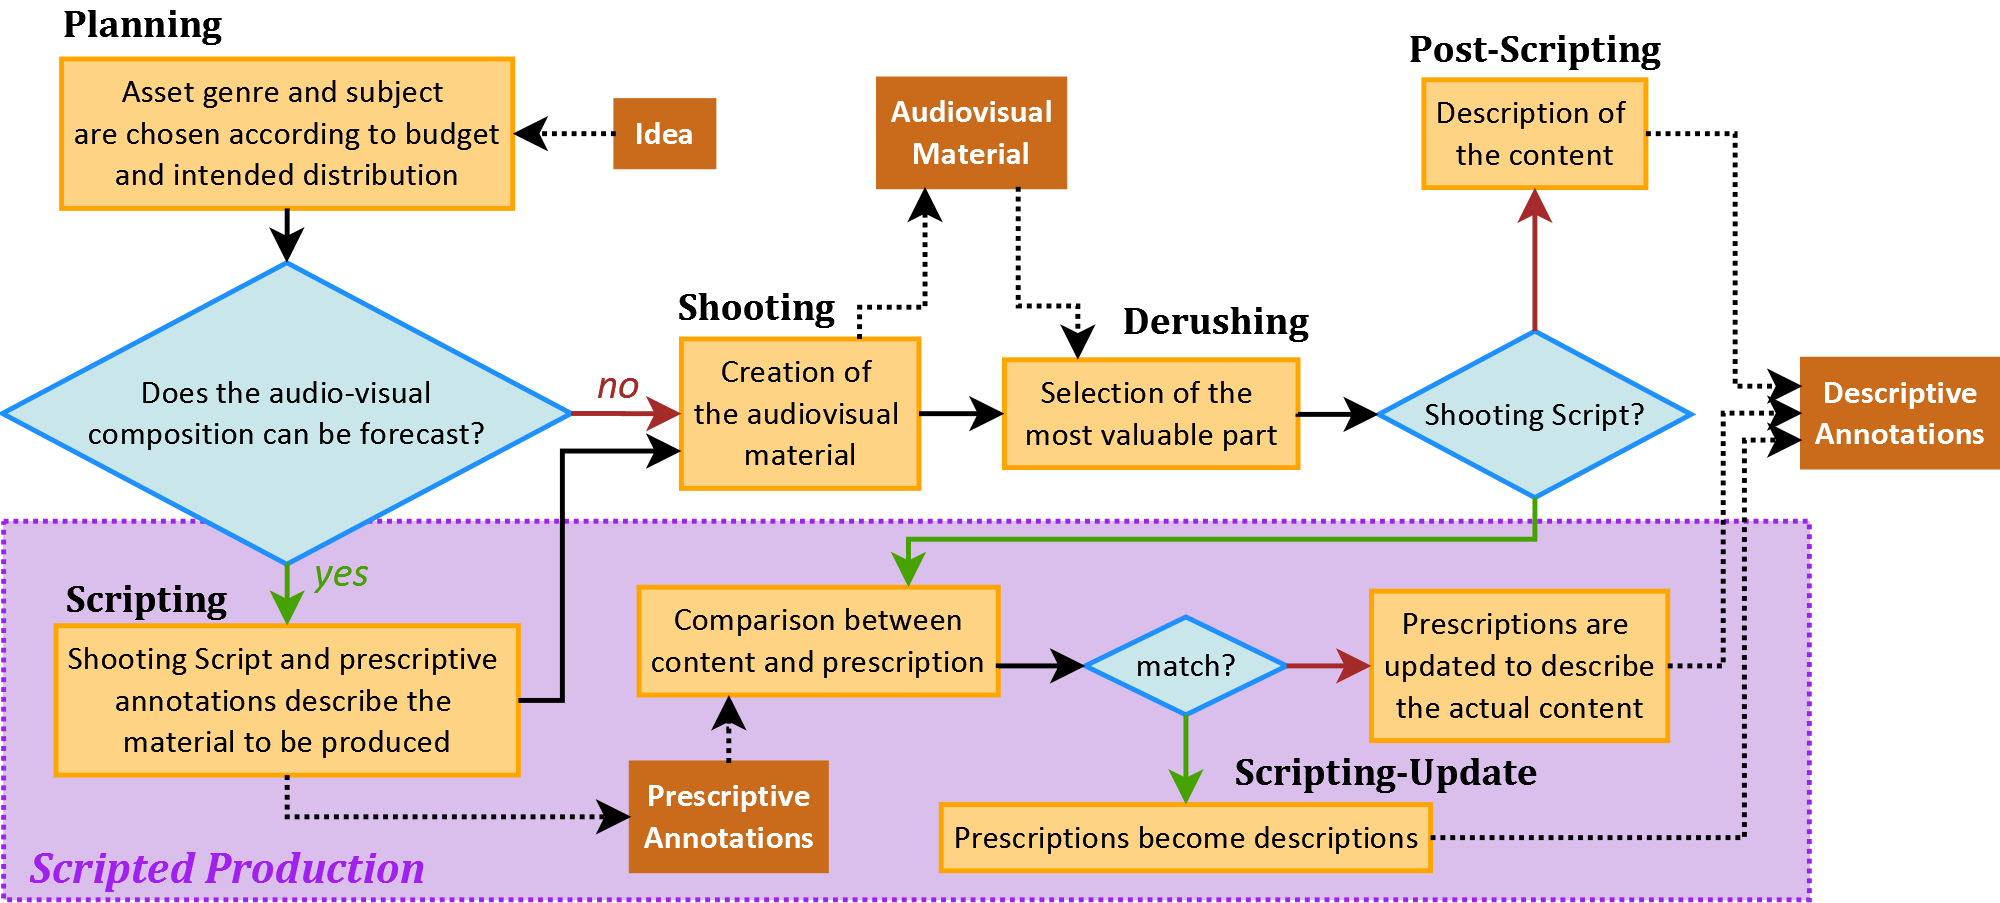
\includegraphics[width=0.9\textwidth]{./images/Approach-Logigram-v2.png}
\caption{Description contributive et continue pour des productions scriptées et non-scriptées}
\label{img:strat-annot}
\end{figure}

La modélisation du vocabulaire de la production audiovisuelle peut avoir des avantages pour les deux types de production présentés, à condition d'adapter sa stratégie de collecte d'information à l'ensemble de la chaîne de production. 
L'objectif est de récolter l'information dès qu'elle est produite, c'est-à-dire à toutes les étapes de la chaîne. 
Les différences entre les processus de production scripté et non-scripté sont présentés dans la Figure \ref{fig:strat-annot}. 
Dans les rectangles marrons, nous avons les résultats ou les éléments initateurs d'une activité (en noir, et décrites dans des rectangles oranges).
Les flèches pleines correspondent au sens de déroulement du logigramme, les flèches en pointillées correspondent aux importation/exportation d'information. 
Enfin, les losanges bleus correspondant à des embranchements logiques (des questions où l'on peut répondre par oui ou non) qui permettent de distinguer les différents cas à traiter.
Au départ, la production est initié par une idée de programme, originale ou non, qui conduit à la plannification de la production.
Lorsque l'idée correspond à un genre audiovisuel, la structure du document audiovisuel correspond à une grammaire particulière qui peut être modélisé. 
Dans le cas d'une production scriptée, la collecte des informations peut commencer par reprendre les informations contenues dans les documents de production, et notamment le script, pour créer des annotations dites \e{prescriptives} (dictant la fabrication du document et du matériel).
Le tournage permet de fabriquer du matériel, qu'il faut ensuite dérusher, c'est-à-dire identifier les différentes prises de vues et sélectionner les meilleurs morceaux. 
Si il existe des annotations prescriptives, alors elles peuvent être utilisé comme point de départ pour la description du matériel.
La comparaison entre ces annotations et le matériel filmé aboutit à deux situations, soit la prescription à été respecté et les annotations deviennent descriptives, soit il faut les modifier pour en faire des annotations descriptives.
Dans le cas de production non-scriptée, la description du contenu commence véritablement après le dérushage.

Il faut remarquer que ce logigramme ne présume pas de la nature de l'agent construisant, vérifiant et mettant à jour les annotations.
Comme nous le fait remarquer \citeauthor{latour:ia}, humains et machines possèdent des capacités distinctes qu'il convient d'associer de manière conjointe :

\begin{cico}
\e{Comprenez-moi, mettre en machine ne signifie pas décontextualiser, mais situer autre part, dans un autre acteur, une portion des compétences nécessaires à l'action. [\dots] Au lieu de considérer des hommes d'un côté et des formalismes de l'autre, considérons plutôt une liste de compétences et cherchons expérimentalement à repérer, dans l'épreuve, lesquelles peuvent être confiées à quel genres d'acteur nouveaux.} \parcite{latour:ia}
\end{cico} 

Nous appelons cette approche de description \g{contributive} et \g{continue} car elle implique une variété de contributeur opérant à toutes les étapes de la chaîne de production pour fabriquer la description d'un document audiovisuel.


\subsection{Architecture de l'approche}